\documentclass[varwidth,border=10pt]{standalone}

\usepackage[aboveskip=1pt,labelfont=bf,labelsep=period,justification=raggedright,singlelinecheck=off]{caption}
\usepackage{amsmath}
\usepackage{tikz}
\usepackage{tikz-cd}
\usetikzlibrary{matrix,arrows,positioning,calc,shapes,arrows.meta}
\usepackage{xstring}
\tikzset{  
	-Latex,auto,node distance =1.5 cm and 1.3 cm, thick,% node distance is the distance between one node to other, where 1.5cm is the length of the edge between the nodes  
	state/.style ={ellipse, draw, minimum width = 0.9 cm}, % the minimum width is the width of the ellipse, which is the size of the shape of vertex in the node graph  
	point/.style = {circle, draw, inner sep=0.18cm, fill, node contents={}},  
	bidirected/.style={Latex-Latex,dashed}, % it is the edge having two directions  
	el/.style = {inner sep=2.5pt, align=right, sloped}  
} 
%\usepackage[subrefformat=parens, labelfont=up]{subcaption}
%\usepackage{cleveref}
%\crefname{thm}{Theorem}{Theorems}
\setlength{\textwidth}{\dimexpr 6in\relax}
\usepackage{makecell}



\newcommand{\bbB}{\mathbb{B}}
\newcommand{\bL}{\mathbb{L}}
\newcommand{\bU}{\mathbb{U}}

\newcommand{\cL}{\mathcal{L}}
\newcommand{\cM}{\mathcal{M}}

\newcommand{\Targets}{\mathbf{T}}
\newcommand{\Sources}{\mathbf{S}}

\newcounter{countitems}


\newcommand{\boolf}{{\mathfrak 0}}
\newcommand{\boolt}{{\mathfrak 1}}

\newcommand{\bzero}{{\bf 0}}
\newcommand{\bone}{{\bf 1}}

\newcommand{\setof}[1]{\left\{ {#1}\right\}}
\newcommand{\setdef}[2]{\left\{{#1}\,\left|\,{#2}\right.\right\}}

\usepackage[subrefformat=parens, labelfont=up]{subcaption}

\begin{document}

\begin{figure}[p]
\centering
\begin{subfigure}[c]{0.6\textwidth}
\centering
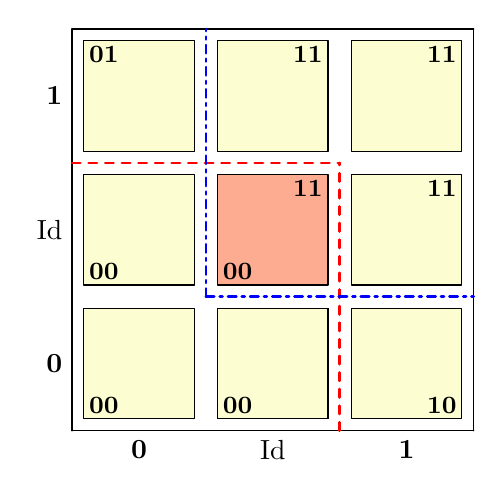
\begin{tikzpicture}[line cap=round,line join=round,every path/.style={-}]
\def\N{3}
\def\cell{1.7}
\def\tile{1.4}
\def\ofs{0.05cm}
\def\labelfont{\normalsize}
\def\gridlw{0.6pt}
\def\thicklw{1.6pt}
\def\boxfont{\small\bfseries}
\definecolor{cellcolor4}{RGB}{133,89,163}
\definecolor{cellcolor3}{RGB}{204,115,161}
\definecolor{cellcolor2}{RGB}{253,172,145}
\definecolor{cellcolor1}{RGB}{253,253,210}
\draw[line width=\gridlw] (0,0) -- (\N*\cell,0);
\draw[line width=\gridlw] (\N*\cell,0) -- (\N*\cell,\N*\cell);
\draw[line width=\gridlw] (\N*\cell,\N*\cell) -- (0,\N*\cell);
\draw[line width=\gridlw] (0,\N*\cell) -- (0,0);
\draw[line width=1pt, dashed, red] (0,2*\cell) -- (2*\cell,2*\cell);
\draw[line width=1pt, dashed, red] (2*\cell,0) -- (2*\cell,2*\cell);
\draw[line width=1pt, dashdotted, blue]    (1*\cell,1*\cell) -- (3*\cell,1*\cell);
\draw[line width=1pt, dashdotted, blue]    (1*\cell,1*\cell) -- (1*\cell,3*\cell);
\foreach [count=\c from 0] \name in {$\mathbf{0}$,Id,$\mathbf{1}$} {
  \node[font=\labelfont, anchor=north] at (\c*\cell+0.5*\cell,0) {\name};
  \node[font=\labelfont, anchor=east] at (0,\c*\cell+0.5*\cell) {\name};
}
\newcommand{\drawBox}[3]{%
  \setcounter{countitems}{0}
  \foreach \i in {#3} {
    \stepcounter{countitems}
  }
  \edef\boxcolor{cellcolor\arabic{countitems}}
  \path let \p1 = (#1*\cell+0.5*\cell,#2*\cell+0.5*\cell) in
    node[draw, fill=\boxcolor, inner sep=0pt,
         minimum width=\tile cm, minimum height=\tile cm] (box-#1-#2) at (\x1,\y1) {};
}
\newcommand{\placeCorner}[3]{%
  \edef\LBL{#1}%
  \IfStrEq{\LBL}{00}{
    \node[anchor=south west,font=\boxfont]
      at ([xshift=-\ofs,yshift=-\ofs] box-#2-#3.south west) {00};
  }{
  \IfStrEq{\LBL}{11}{
    \node[anchor=north east,font=\boxfont]
      at ([xshift=\ofs,yshift=\ofs] box-#2-#3.north east) {11};
  }{
  \IfStrEq{\LBL}{01}{
    \node[anchor=north west,font=\boxfont]
      at ([xshift=-\ofs,yshift=\ofs] box-#2-#3.north west) {01};
  }{
  \IfStrEq{\LBL}{10}{
    \node[anchor=south east,font=\boxfont]
      at ([xshift=\ofs,yshift=-\ofs] box-#2-#3.south east) {10};
  }{
    \node at (box-#2-#3) {\LBL};
  }}}}%
}
\newcommand{\boxWithLabels}[3]{%
  \drawBox{#1}{#2}{#3}%
  \foreach \lab in {#3} { \placeCorner{\lab}{#1}{#2} }%
}
\boxWithLabels{0}{0}{00}
\boxWithLabels{1}{0}{00}
\boxWithLabels{2}{0}{10}
\boxWithLabels{0}{1}{00}
\boxWithLabels{1}{0}{00}
\boxWithLabels{1}{1}{00,11}
\boxWithLabels{2}{1}{11}
\boxWithLabels{0}{2}{01}
\boxWithLabels{1}{2}{11}
\boxWithLabels{2}{2}{11}
\end{tikzpicture}
\caption{}
\label{fig:PG1}
\end{subfigure}
\begin{subfigure}[c]{0.35\textwidth}
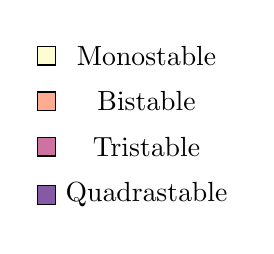
\begin{tikzpicture}
\definecolor{cellcolor4}{RGB}{133,89,163}
\definecolor{cellcolor3}{RGB}{204,115,161}
\definecolor{cellcolor2}{RGB}{253,172,145}
\definecolor{cellcolor1}{RGB}{253,253,210}
\matrix[column sep=0cm, row sep=0.1cm] {
\node[draw, fill=cellcolor1, minimum width=0.1cm, minimum height=0.1cm] {}; & \node {Monostable}; \\
\node[draw, fill=cellcolor2, minimum width=0.1cm, minimum height=0.1cm] {}; & \node {Bistable}; \\
\node[draw, fill=cellcolor3, minimum width=0.1cm, minimum height=0.1cm] {}; & \node {Tristable}; \\
\node[draw, fill=cellcolor4, minimum width=0.1cm, minimum height=0.1cm] {}; & \node {Quadrastable}; \\
};
\end{tikzpicture}
\end{subfigure}
\vskip0.2in
\begin{subfigure}{0.9\textwidth}
\centering
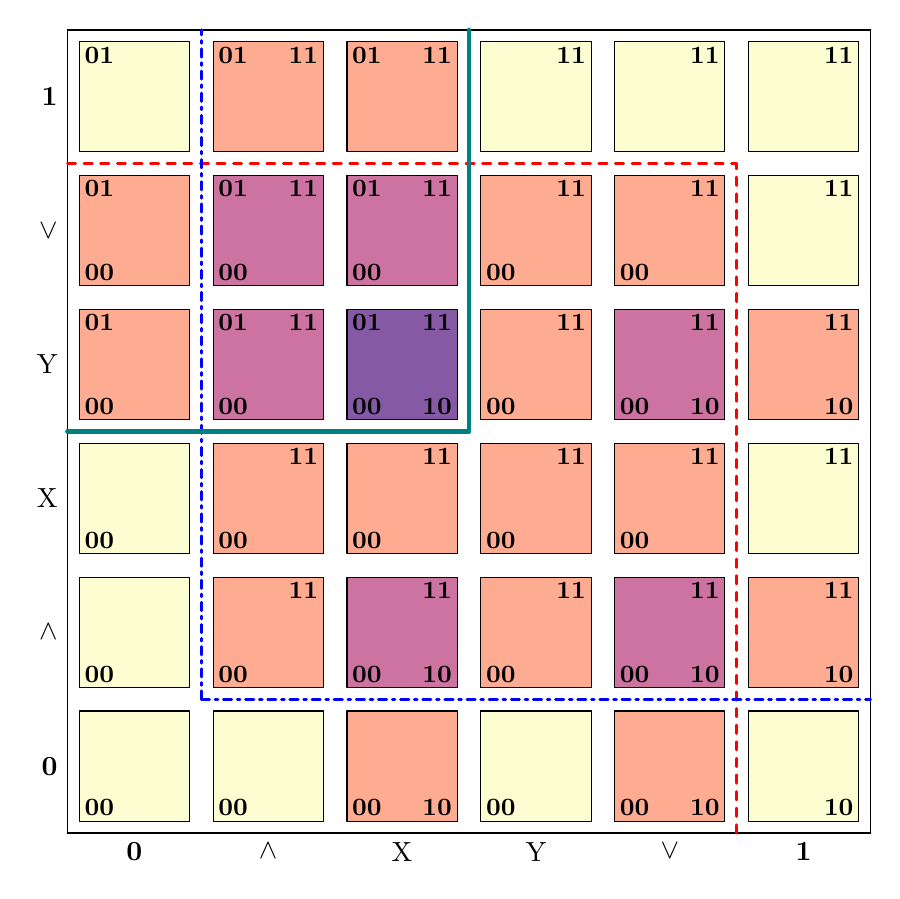
\begin{tikzpicture}[line cap=round,line join=round,every path/.style={-}]

\def\N{6}
\def\cell{1.7}
\def\tile{1.4}
\def\ofs{0.05cm}
\def\labelfont{\normalsize}
\def\gridlw{0.6pt}
\def\thicklw{1.6pt}
\def\boxfont{\small\bfseries}
\definecolor{cellcolor4}{RGB}{133,89,163}
\definecolor{cellcolor3}{RGB}{204,115,161}
\definecolor{cellcolor2}{RGB}{253,172,145}
\definecolor{cellcolor1}{RGB}{253,253,210}
\draw[line width=\gridlw] (0,0) -- (\N*\cell,0);
\draw[line width=\gridlw] (\N*\cell,0) -- (\N*\cell,\N*\cell);
\draw[line width=\gridlw] (\N*\cell,\N*\cell) -- (0,\N*\cell);
\draw[line width=\gridlw] (0,\N*\cell) -- (0,0);
\draw[line width=1pt, dashed, red] (0,5*\cell) -- (5*\cell,5*\cell);
\draw[line width=1pt, dashed, red] (5*\cell,0) -- (5*\cell,5*\cell);
\draw[line width=1pt, dashdotted, blue]    (1*\cell,1*\cell) -- (6*\cell,1*\cell);
\draw[line width=1pt, dashdotted, blue]    (1*\cell,1*\cell) -- (1*\cell,6*\cell);
\draw[line width=\thicklw, teal]    (3*\cell,6*\cell) -- (3*\cell,3*\cell);
\draw[line width=\thicklw, teal]    (0*\cell,3*\cell) -- (3*\cell,3*\cell);
\foreach [count=\c from 0] \name in {$\mathbf{0}$,$\wedge$,X,Y,$\vee$,$\mathbf{1}$} {
  \node[font=\labelfont, anchor=north] at (\c*\cell+0.5*\cell,0) {\name};
  \node[font=\labelfont, anchor=east] at (0,\c*\cell+0.5*\cell) {\name};
}
\newcommand{\drawBox}[3]{%
  \setcounter{countitems}{0}
  \foreach \i in {#3} {
    \stepcounter{countitems}
  }
  \edef\boxcolor{cellcolor\arabic{countitems}}
  \path let \p1 = (#1*\cell+0.5*\cell,#2*\cell+0.5*\cell) in
    node[draw, fill=\boxcolor, inner sep=0pt,
         minimum width=\tile cm, minimum height=\tile cm] (box-#1-#2) at (\x1,\y1) {};
}
\newcommand{\placeCorner}[3]{%
  \edef\LBL{#1}%
  \IfStrEq{\LBL}{00}{
    \node[anchor=south west,font=\boxfont]
      at ([xshift=-\ofs,yshift=-\ofs] box-#2-#3.south west) {00};
  }{
  \IfStrEq{\LBL}{11}{
    \node[anchor=north east,font=\boxfont]
      at ([xshift=\ofs,yshift=\ofs] box-#2-#3.north east) {11};
  }{
  \IfStrEq{\LBL}{01}{
    \node[anchor=north west,font=\boxfont]
      at ([xshift=-\ofs,yshift=\ofs] box-#2-#3.north west) {01};
  }{
  \IfStrEq{\LBL}{10}{
    \node[anchor=south east,font=\boxfont]
      at ([xshift=\ofs,yshift=-\ofs] box-#2-#3.south east) {10};
  }{
    \node at (box-#2-#3) {\LBL};
  }}}}%
}
\newcommand{\boxWithLabels}[3]{%
  \drawBox{#1}{#2}{#3}%
  \foreach \lab in {#3} { \placeCorner{\lab}{#1}{#2} }%
}
\boxWithLabels{0}{0}{00}
\boxWithLabels{1}{0}{00}
\boxWithLabels{2}{0}{00,10}
\boxWithLabels{3}{0}{00}
\boxWithLabels{4}{0}{00,10}
\boxWithLabels{5}{0}{10}
\boxWithLabels{0}{1}{00}
\boxWithLabels{1}{1}{11,00}
\boxWithLabels{2}{1}{11,00,10}
\boxWithLabels{3}{1}{11,00}
\boxWithLabels{4}{1}{11,00,10}
\boxWithLabels{5}{1}{11,10}
\boxWithLabels{0}{2}{00}
\boxWithLabels{1}{2}{11,00}
\boxWithLabels{2}{2}{11,00}
\boxWithLabels{3}{2}{11,00}
\boxWithLabels{4}{2}{11,00}
\boxWithLabels{5}{2}{11}
\boxWithLabels{0}{3}{01,00}
\boxWithLabels{1}{3}{01,11,00}
\boxWithLabels{2}{3}{01,11,00,10}
\boxWithLabels{3}{3}{11,00}
\boxWithLabels{4}{3}{11,00,10}
\boxWithLabels{5}{3}{11,10}
\boxWithLabels{0}{4}{01,00}
\boxWithLabels{1}{4}{01,11,00}
\boxWithLabels{2}{4}{01,11,00}
\boxWithLabels{3}{4}{11,00}
\boxWithLabels{4}{4}{11,00}
\boxWithLabels{5}{4}{11}
\boxWithLabels{0}{5}{01}
\boxWithLabels{1}{5}{01,11}
\boxWithLabels{2}{5}{01,11}
\boxWithLabels{3}{5}{11}
\boxWithLabels{4}{5}{11}
\boxWithLabels{5}{5}{11}
\end{tikzpicture}
\caption{}
\label{fig:PG2}
\end{subfigure}
\label{fig:PG}
\end{figure}

\end{document}